\documentclass[12pt]{article}
\usepackage[brazil]{babel}
\usepackage[utf8]{inputenc}
\usepackage{amsmath}
\usepackage{amsfonts}
\usepackage{amssymb}
\usepackage{geometry}
\usepackage{graphicx}
\usepackage{float}
\usepackage{enumitem}
\usepackage{multicol}
\usepackage{array}
\usepackage{xcolor}
\usepackage{siunitx}
\usepackage{url}


\usepackage[T1]{fontenc}
\usepackage{mathptmx} %times new roman


\geometry{a4paper, margin=1.2cm}
\setlength{\parindent}{0cm}

\begin{document}

% -------------------- CABEÇALHO ----------------------
\thispagestyle{empty}
\vspace{0.5cm}
\begin{center}
	\large
	\begin{tabular}{|l l|}
		\hline
		\textbf{ESCOLA:} & EETI GILBERTO MESTRINHO DE MEDEIROS RAPOSO \\ 
		\textbf{ALUNA(O):} & \underline{\hspace{7cm}} \textbf{SÉRIE:} \underline{\hspace{1.5cm}} \textbf{TURMA:} \underline{\hspace{1.5cm}} \\
		\textbf{PROFESSOR:} & \underline{\hspace{7cm}} \textbf{DATA:} \underline{\hspace{1.5cm}}/\underline{\hspace{1.5cm}}/\underline{\hspace{1.5cm}} \\
		\textbf{VALOR:} & \underline{\hspace{3cm}} \textbf{NOTA:} \underline{\hspace{1.5cm}} \\
		\hline
	\end{tabular}
\end{center}
\vspace{0.5cm}

\vspace{0.4cm}

\begin{center}
\Large \textbf{LISTA DE EXERCÍCIOS SOBRE FUNÇÕES TRIGONOMÉTRICAS}
\end{center}

\vspace{0.2cm}

\textbf{ATENÇÃO:}
\begin{itemize}
    \item Resolva toda a lista, justificando cada questão.
    \item Coloque o nome completo e identificação no cabeçalho.
    \item Faça na lista, se e somente se a resolução de cada questão couber em cada questão.
    \item Há apenas uma opção correta em cada questão de múltipla escolha.
    \item Caso opte por fazer numa folha à parte, identifique cada questão.
\end{itemize}

\vspace{0.4cm}

% -------------------- QUESTÕES EM DUAS COLUNAS ----------------------
\begin{multicols}{2}

% -------- QUESTÃO 1 ---------
\textbf{Questão 1 - SIS} \\

Considere o gráfico da função trigonométrica \(f(x) = a \cdot \cos x + b\), em que \(a\) e \(b\) são constantes reais.

\begin{center}

    \centering
    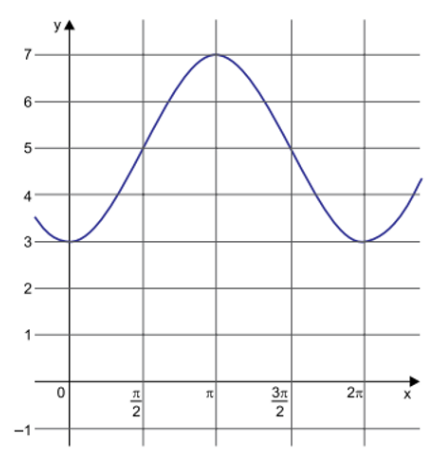
\includegraphics[width=0.8\linewidth]{imagens/função1.png}

\end{center}

O valor de \(a + b\) é igual a:

\begin{itemize}
    \item[(A)] 3
    \item[(B)] 4
    \item[(C)] 5
    \item[(D)] 7
    \item[(E)] 10
\end{itemize}

\vspace{0.3cm}

% -------- QUESTÃO 2 ---------
\textbf{Questão 2 - SIS} \\

Considere o gráfico de uma função trigonométrica \(f\) tal que:

\[
-3 \leq f(x) \leq 1
\]

para todo \(x \in \mathbb{R}\), conforme mostra a figura:

\begin{center}

    \centering
    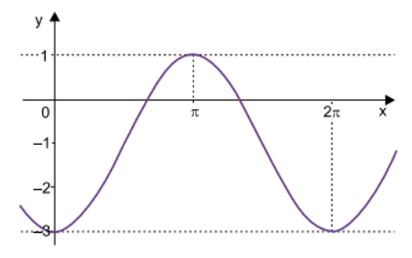
\includegraphics[width=0.8\linewidth]{imagens/image.png}

\end{center}

A função \(f\) pode ser representada por:

\begin{itemize}
    \item[(A)] \(f(x) = -2\cos(x) - 1\)
    \item[(B)] \(f(x) = \cos(x) - 2\)
    \item[(C)] \(f(x) = -3\operatorname{tg}(x) + 1\)
    \item[(D)] \(f(x) = 2\operatorname{sen}(x) - 3\)
    \item[(E)] \(f(x) = -3\operatorname{sen}(x) + 1\)
\end{itemize}
% -------- QUESTÃO 3 ---------
\textbf{Questão 3 - SIS} \\

A imagem da função

\[
y = \frac{6}{2 - sen(2x)}
\]

é:

\begin{itemize}
    \item[(A)] \(\{y \in \mathbb{R} \, | \, 1 \leq y \leq 3\}\)
    \item[(B)] \(\{y \in \mathbb{R} \, | \, 2 \leq y \leq 3\}\)
    \item[(C)] \(\{y \in \mathbb{R} \, | \, 2 \leq y \leq 6\}\)
    \item[(D)] \(\{y \in \mathbb{R} \, | \, 3 \leq y \leq 6\}\)
    \item[(E)] \(\{y \in \mathbb{R} \, | \, 3 \leq y \leq 12\}\)
\end{itemize}

\vspace{0.3cm}

% -------- QUESTÃO 4 ---------
\textbf{Questão 4 - SIS} \\

O gráfico da função

\[
f(x) = a + b \cdot sen\left(c \cdot x - \frac{\pi}{2}\right)
\]

em que \(a\), \(b\) e \(c\) são constantes reais, está representado na figura:

\begin{center}

    \centering
    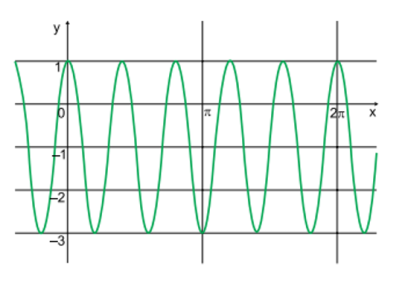
\includegraphics[width=0.8\linewidth]{imagens/função3.png}

\end{center}

O valor do produto \(abc\) é igual a:

\begin{itemize}
    \item[(A)] 10
    \item[(B)] 5
    \item[(C)] 2
    \item[(D)] -4
    \item[(E)] -6
\end{itemize}
% -------- QUESTÃO 5 ---------
\textbf{Questão 5 - SIS} \\

Considere o gráfico da função

\[
f(x) = \frac{sen(4x)}{4}
\]

No intervalo fechado \([0, 2\pi]\), o número de vezes que o gráfico de \(f\) intersecta o eixo \(x\) é:

\begin{itemize}
    \item[(A)] 1
    \item[(B)] 3
    \item[(C)] 5
    \item[(D)] 7
    \item[(E)] 9
\end{itemize}

\vspace{0.3cm}

% -------- QUESTÃO 6 ---------
\textbf{Questão 6 - SIS} \\

A temperatura superficial da água de um lago, em determinada época do ano, varia no decorrer das horas do dia, de acordo com a função

\[
T(t) = 20 + 5 \cdot sen\left( \frac{\pi}{4} \cdot t \right)
\]

em que \(T\) é a temperatura da superfície do lago em \(^\circ C\) e \(t\) é a hora do dia (com \(0 \leq t \leq 8\) e \(t = 0\) correspondendo ao meio-dia, \(t = 1\) às 13 horas e assim sucessivamente).

Considerando essas informações, a temperatura máxima e a hora do dia em que ela ocorrerá será:

\begin{itemize}
    \item[(A)] 20\(^\circ C\) às 12 horas
    \item[(B)] 20\(^\circ C\) às 14 horas
    \item[(C)] 22\(^\circ C\) às 12 horas
    \item[(D)] 25\(^\circ C\) às 14 horas
    \item[(E)] 25\(^\circ C\) às 15 horas
\end{itemize}
% -------- QUESTÃO 7 ---------
\textbf{Questão 7 - MACRO} \\

Considere a função 

\[
f(x) = 5 - \sqrt{2} \cdot \cos\left( \frac{x}{4} \right)
\]

O valor de \(f(\pi)\) é igual a:

\begin{itemize}
    \item[(A)] 1
    \item[(B)] 5
    \item[(C)] 4
    \item[(D)] 2
    \item[(E)] 3
\end{itemize}

\vspace{0.3cm}

% -------- QUESTÃO 8 ---------
\textbf{Questão 8 - MACRO} \\

Considere a função 

\[
f(x) = 4 \cdot sen(2x)
\]

O valor de 

\[
f\left( \frac{\pi}{3} \right)
\]

é:

\begin{itemize}
    \item[(A)] \(\frac{\sqrt{2}}{2}\)
    \item[(B)] \(\frac{\sqrt{3}}{2}\)
    \item[(C)] \(2\sqrt{3}\)
    \item[(D)] \(2\sqrt{2}\)
    \item[(E)] \(\sqrt{3}\)
\end{itemize}
% -------- QUESTÃO 9 ---------
\textbf{Questão 9 - MACRO} \\

A função 

\[
f(x) = 1 - sen(x)
\]

está representada pelo gráfico:

\begin{center}


    \centering
    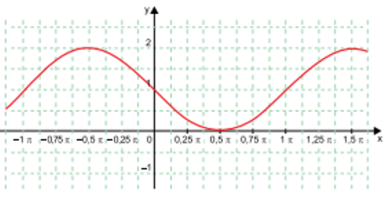
\includegraphics[width=0.8\linewidth]{imagens/função5.png}

    \centering
    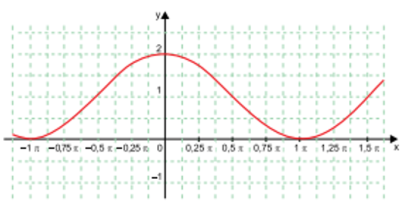
\includegraphics[width=0.8\linewidth]{imagens/função6.png}

    \centering
    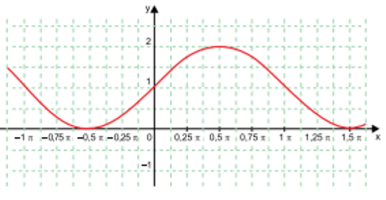
\includegraphics[width=0.8\linewidth]{imagens/função7.png}

    \centering
    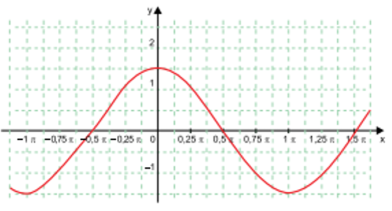
\includegraphics[width=0.8\linewidth]{imagens/função8.png}

    \centering
    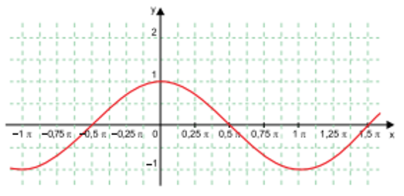
\includegraphics[width=0.8\linewidth]{imagens/função9.png}

\end{center}

\begin{itemize}
    \item[(A)] Gráfico (A)
    \item[(B)] Gráfico (B)
    \item[(C)] Gráfico (C)
    \item[(D)] Gráfico (D)
    \item[(E)] Gráfico (E)
\end{itemize}

\vspace{0.3cm}

% -------- QUESTÃO 10 ---------
\textbf{Questão 10 - MACRO} \\

Analise o gráfico.

\begin{center}

    \centering
    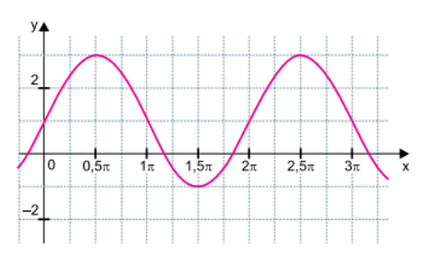
\includegraphics[width=0.8\linewidth]{imagens/função10.png}

\end{center}

A função descrita pelo gráfico pode ser dada por:

\begin{itemize}
    \item[(A)] \(f(x) = 1 + 2sen(x)\)
    \item[(B)] \(f(x) = 2sen(x)\)
    \item[(C)] \(f(x) = 1 + sen(x)\)
    \item[(D)] \(f(x) = sen(x)\)
    \item[(E)] \(f(x) = 2 - sen(x)\)
\end{itemize}

% -------- QUESTÃO 11 ---------
\textbf{Questão 11} \\

Dada a função 

\[
f(x) = \sin(x) + 3
\]

o valor numérico da função para 

\[
x = \frac{3\pi}{2}
\]

é:

\begin{itemize}
    \item[(A)] 0
    \item[(B)] 1
    \item[(C)] 2
    \item[(D)] 3
    \item[(E)] 4
\end{itemize}

\vspace{0.3cm}

% -------- QUESTÃO 12 ---------
\textbf{Questão 12} \\

Conhecendo a função 

\[
f(x) = 4\cos(2x) + 1
\]

podemos afirmar que a imagem da função é igual a:

\begin{itemize}
    \item[(A)] \([-2, 2]\)
    \item[(B)] \([-3, 5]\)
    \item[(C)] \([-1, 1]\)
    \item[(D)] \([-4, 8]\)
    \item[(E)] \(]-\infty, \infty[\)
\end{itemize}
% -------- QUESTÃO 13 ---------
\textbf{Questão 13} \\

Dada a função trigonométrica a seguir:

\[
f(x) = \frac{1}{4 - sen(x)}
\]

Podemos afirmar que o menor valor que \(f(x)\) pode assumir é:

\begin{itemize}
    \item[(A)] \(\frac{1}{3}\)
    \item[(B)] \(\frac{1}{4}\)
    \item[(C)] \(\frac{1}{5}\)
    \item[(D)] \(-\frac{1}{4}\)
    \item[(E)] -1
\end{itemize}

\vspace{0.3cm}

% -------- QUESTÃO 14 ---------
\textbf{Questão 14} \\

Analise o gráfico da função trigonométrica a seguir:

\begin{center}

    \centering
    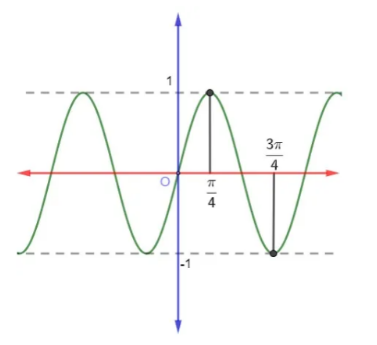
\includegraphics[width=0.8\linewidth]{imagens/função11.png}

\end{center}

A lei de formação que descreve a função demonstrada no gráfico é:

\begin{itemize}
    \item[(A)] \(f(x) = sen(x)\)
    \item[(B)] \(f(x) = cos(x)\)
    \item[(C)] \(f(x) = sen(2x)\)
    \item[(D)] \(f(x) = cos(2x)\)
    \item[(E)] \(f(x) = 2tg(x)\)
\end{itemize}
% -------- QUESTÃO 15 ---------
\textbf{Questão 15} \\

Dada a função 

\[
f(x) = 1 + 2\cos(x)
\]

seja \(x\) um ângulo do primeiro quadrante. Então, o valor de \(x\) que faz com que \(f(x) = 2\) é:

\begin{itemize}
    \item[(A)] \(\pi\)
    \item[(B)] \(\frac{\pi}{6}\)
    \item[(C)] \(\frac{\pi}{5}\)
    \item[(D)] \(\frac{\pi}{4}\)
    \item[(E)] \(\frac{\pi}{3}\)
\end{itemize}

\vspace{0.3cm}

% -------- QUESTÃO 16 ---------
\textbf{Questão 16} \\

Dada a função

\[
f(x) = sen^{2}(x) + 2\cos(x)
\]

o valor numérico da função para 

\[
x = \frac{\pi}{4}
\]

é:

\begin{itemize}
    \item[(A)] \(0,5 + \sqrt{2}\)
    \item[(B)] \(1 + \sqrt{2}\)
    \item[(C)] 4
    \item[(D)] \(4 - \sqrt{2}\)
    \item[(E)] \(0,5 + \sqrt{3}\)
\end{itemize}
% -------- QUESTÃO 17 ---------
\textbf{Questão 17 - Cefet-PR} \\

A função real 

\[
f(x) = a + b \cdot sen(c \cdot x)
\]

tem imagem igual a \([-7, 9]\) e seu período é \(\frac{\pi}{2}\) rad. Assim, \(a + b + c\) vale:

\begin{itemize}
    \item[(A)] 13
    \item[(B)] 9
    \item[(C)] 8
    \item[(D)] -4
    \item[(E)] 10
\end{itemize}

\vspace{0.3cm}

% -------- QUESTÃO 18 ---------
\textbf{Questão 18 - UFRGS} \\

Considere as funções \(f\) e \(g\) definidas por:

\[
f(x) = sen(x) \quad \text{e} \quad g(x) = \cos(x)
\]

O número de raízes da equação \(f(x) = g(x)\) no intervalo \([-2\pi, 2\pi]\) é:

\begin{itemize}
    \item[(A)] 3
    \item[(B)] 4
    \item[(C)] 5
    \item[(D)] 6
    \item[(E)] 7
\end{itemize}
% -------- QUESTÃO 19 ---------
\textbf{Questão 19 - UNITAU} \\

O período da função

\[
y = sen\left( \frac{\pi}{\sqrt{2}} \cdot x \right)
\]

é:

\begin{itemize}
    \item[(A)] \(\frac{\sqrt{2}}{2}\)
    \item[(B)] \(\frac{\sqrt{\pi}}{2}\)
    \item[(C)] \(\frac{\pi}{2}\)
    \item[(D)] \(\sqrt{2}\)
    \item[(E)] \(\frac{\sqrt{2}}{2}\)
\end{itemize}
% -------- QUESTÃO 20 ---------
\textbf{Questão 20 - PUC-RS} \\

Dois amigos caminham no plano \(xy\), ao longo de retas paralelas cujas equações são:

\[
2x + 5y = 7 \quad \text{e} \quad 3x + my = 1
\]

Então, o valor de \(m\) é:

\begin{itemize}
    \item[(A)] \(\frac{17}{2}\)
    \item[(B)] \(\frac{15}{2}\)
    \item[(C)] \(\frac{19}{2}\)
    \item[(D)] \(\frac{13}{2}\)
    \item[(E)] \(\frac{11}{2}\)
\end{itemize}
% -------- QUESTÃO 21 ---------
\textbf{Questão 21 - UESB-BA} \\

A reta perpendicular à reta 
\[
r: 2x + 3y = 1
\]

no ponto em que \(r\) intercepta o eixo das abscissas, pode ser descrita pela equação:

\begin{itemize}
    \item[(A)] \(6x - 4y = 3\)
    \item[(B)] \(4y - 6x = 3\)
    \item[(C)] \(6x + 4y = -3\)
    \item[(D)] \(3x - 2y = 1\)
    \item[(E)] \(2x - 3y = 1\)
\end{itemize}
% -------- QUESTÃO 22 ---------


\textbf{Questão 22} \\

Quando há duas retas pertencentes ao mesmo plano, elas podem ter três posições possíveis. A seguir, faça a correspondência correta entre os tipos de reta e suas respectivas características:

\begin{itemize}
    \item I. Concorrentes
    \item II. Coincidentes
    \item III. Paralelas
\end{itemize}

\begin{itemize}
    \item ( \, ) têm infinitos pontos em comum.
    \item ( \, ) têm um único ponto em comum.
    \item ( \, ) não têm nenhum ponto em comum.
\end{itemize}

Agora marque a alternativa que representa a correspondência correta:

\begin{itemize}
    \item[(A)] I, II e III
    \item[(B)] II, III e I
    \item[(C)] II, I e III
    \item[(D)] III, II e I
    \item[(E)] III, I e II
\end{itemize}

\textbf{Questão 23} \\

	Um recipiente tem um formato que faz com que, ao ser enchido de água com uma vazão constante, a distância D da lâmina de água ao tampo da mesa, em centímetro, aumente em relação ao tempo T, em minuto, de acordo com uma função do tipo $$D=k+\tan \left[p.\left(T+m \right)  \right]$$ sendo os parâmetros k, p e m números reais, para T variando entre 0 e 4 minutos, conforme ilustrado na figura, na qual estão apresentadas assíntotas verticais da função tangente utilizada na definição de D.
	
	\begin{center}
		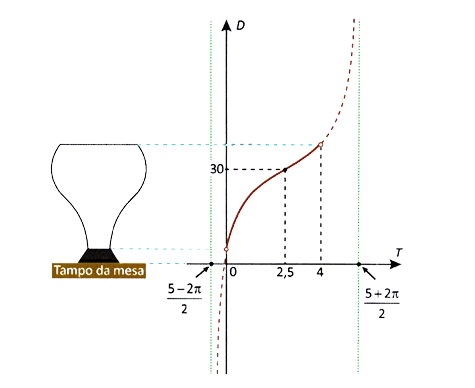
\includegraphics[scale=0.5]{imagens/funcao_tangente.png}
	\end{center} A expressão algébrica que representa a relação entre D e T é 
	
	\begin{itemize}
		\item[(A)] $D=2,5+\tan \left[ 30\left( T - \dfrac{5-2\pi}{2} \right) \right] $\\
		\item[(B)] $D=4+\tan \left[ 30\left( T + \dfrac{5}{2} \right) \right] $\\
		\item[(C)] $D=4+\tan \left[ 2,5\left( T + \dfrac{5+2\pi}{2} \right) \right] $\\
		\item[(D)] $D=30+\tan \left[\dfrac{1}{2}\left( T -5 \right) \right] $\\
		\item[(E)] $D=30+\tan \left[\dfrac{1}{2}\left( T - \dfrac{5}{2} \right) \right] $\\ %
	\end{itemize}

\end{multicols}

\end{document}